\chapter{Strain-induced vector potentials: Lattice-corrections and engineered pseudo magnetic fields\label{chap:PVP}}

At the intersection of graphene's outstanding mechanical and electrical properties lies a peculiar and provocative coupling.
Certain strain distributions in graphene can trick the electrons into acting as if they were in a magnetic field.
Strain shifts the crystal momentum of the Dirac points much like the the canonical momentum is shifted in the presence of a magnetic field.
This exotic coupling is made more appealing by the two dimensional elastic nature of graphene.
Not only does the coupling exist in theory, but the material also allows the physical realization of it.

A dazzling glimpse of the feasibility and potential of strain-engineered graphene \cite{Pereira2009a,Guinea2009} has recently emerged with experiments reporting that certain strain profiles can induce Landau quantization and effective pseudomagnetic fields in excess of 300 T \cite{Levy2010,Yan2012,Yeh2011}.
This strongly encourages the prospect of harnessing this unconventional interplay between electronic and mechanical properties to control electronic transport in graphene devices \cite{Pereira2009a,Fogler2008}.

This chapter starts by discussing the theory of the strain-induced vector potentials with an emphasis on the lattice-corrections first introduced by the author \cite{Kitt2012,Kitt2013}.
This is followed by an examination of the importance of these lattice-corrections in different physical scenarios.
Finally, methods of strain engineering graphene devices are examined with an emphasis on the over pressured hour glass shaped microchamber.
This device cleverly takes advantage of plasmonics to enhance signals from high pseudo magnetic field regions.

\section{Derivation of the pseudo vector potentials}

By distorting the graphene lattice, strain causes the following \cite{Pereira2009}:
(i) for any amount of strain, the Dirac points are displaced from the corners of the unstrained BZ and, furthermore, do not necessarily sit at the corners of the strained BZ;
(ii) the gapless and conical nature of the energy dispersion remains robust, except when the deformation is so strong that the two inequivalent Dirac points merge in a Lifshitz transition (but that probably requires strains of the order 20\%, where the tight-binding description is not reliable anymore);
(iii) at any finite density the Fermi line is deformed from an isotropic circle to an elliptical shape, and two Fermi velocities can be defined along the principal directions \cite{Pereira2009,Pereira2010c,Choi2010}.
All these modifications are significant and happen concurrently. 

From the theoretical as well as technical point of view, the effects of strain are frequently considered independently.
One usually isolates the dominant effect for the physical observable of interest.
For example, the strain-induced corrections to optical absorption arising from inter-band transitions are insensitive to the absolute position of the Dirac point in the BZ (i), but strongly depend on the velocity anisotropy (iii) \cite{Pereira2010c,Pellegrino2010}.
On the other hand, the local shift of the Dirac point (i) can hinder or completely suppress electronic propagation across regions of different strain states \cite{Pereira2009a,Fogler2008}.
In a first approach the anisotropy (iii) is usually neglected in these situations\cite{Fogler2008,Pereira2009a}.

When the strain-induced shift of the Dirac points (i) is considered independently of (ii) and (iii), it can be thought of as a pseudo vector potential \cite{Sasaki2005,Ando2006,Manes2007,CastroNeto2009,Vozmediano2010}.
This can be done because of the peculiar form of the strain corrections to the electronic dispersion in graphene.
Electrons in strained graphene are still governed by a Dirac equation, but one in which the strain modifications can be completely absorbed in the replacement $\hbar \vec{k} \to \hbar \vec{k}-e \vec{\mathcal{A}}$ where $\vec{\mathcal{A}}$ is the pseudo vector potential.
This matches the conventional minimal coupling scenario used to describe electronics in a magnetic field.
The strains response maps onto the response to a magnetic field, and thus, electrons in strained graphene can behave as if they were in a magnetic field.  
The pseudo vector potential is related to the shift in the Dirac point, $\Delta \vec{k}_D$, through $\Delta \vec{k}_D=-\frac{e}{\hbar} \vec{\mathcal{A}}$.

An omission in earlier work in the context of these pseudo vector potentials is the explicit consideration of the deformation of the lattice when computing the position of the new Dirac points.
Here this effect is included and its importance in determining the pseudo vector potentials is shown.
The inclusion of the lattice deformation yields new leading order terms in the strain-induced pseudo vector potential which are different at the three inequivalent Dirac points.
The discussion is restricted to planar deformations, and hence ignore effects that might arise in the presence of curvature \cite{CastroNeto2009,Vozmediano2010}.
A detailed derivation of the pseudo vector potential will be presented.
It will begin with a geometric motivation of the strain-induced perturbations, continue by determining the strain dependencies of these perturbations, and finish with the derivation of the pseudo vector potentials.

\subsection{Strain altered lattice}
The key elements underlying strain-induced pseudo vector potentials are captured by generalizing the tight binding Hamiltonian discussed in Chapter \ref{chap:TB} to the geometry of strained graphene.
Figure \ref{fig:PVP:lattice} illustrates the changes in the lattice geometry due to strain by comparing the unstrained graphene lattice (top row) to the lattice under 20\% uniaxial strain (bottom row).
The large, 20\% strain was chosen to better illustrate the deformation of the lattice and the BZ.
Strain does not need to be this large; all of the effects discussed here are linear in strain.
The method of calculating the distortion of the real and reciprocal space lattices is discussed in detail later in this chapter.
Figure \ref{fig:PVP:lattice} will provide a qualitative geometric picture for how strain modifies the unstrained nearest neighbor tight binding approach discussed in Chapter \ref{chap:TB}.

\begin{figure}
  % Geometry taken directly from my lectures notes on tight binding in graphene
\newcommand{\alat}{1 cm}
\newcommand{\sqth}{1.73205080757}
\newcommand{\Klen}{2 cm}
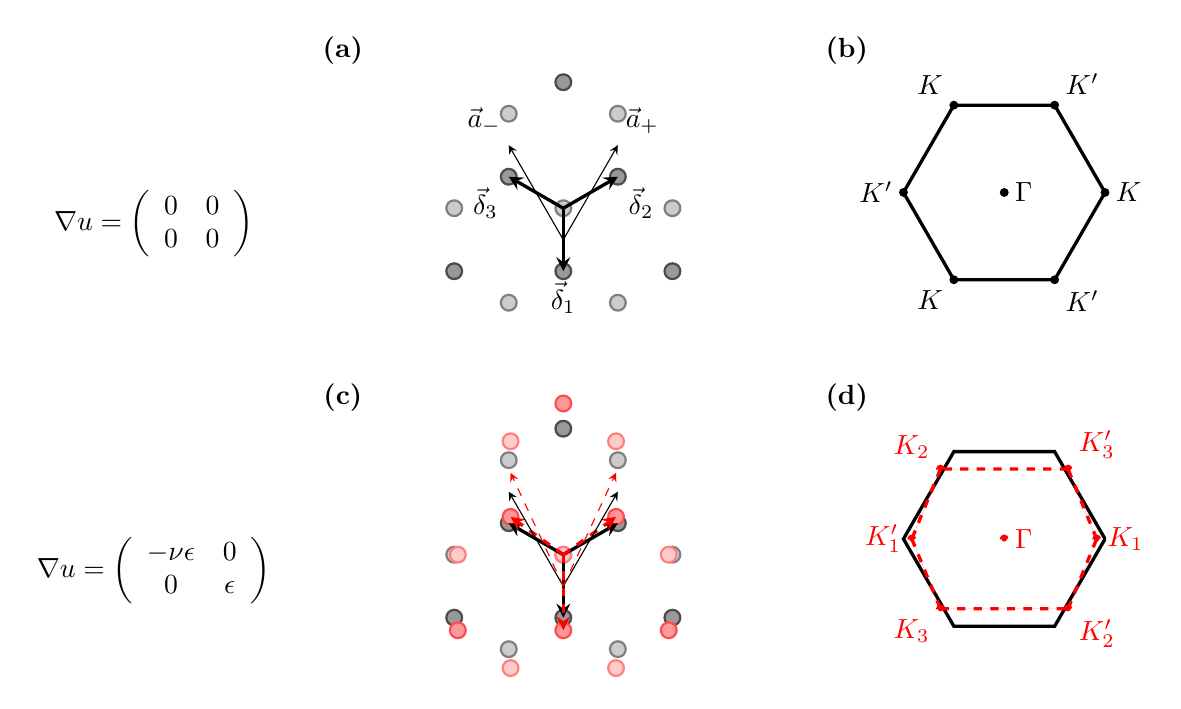
\begin{tikzpicture}[>=stealth,scale=.8,
		nnarrow/.style={color=black,very thick, ->},					% Nearest neighbor vectors
		nnarrows/.style={color=red,very thick, dashed, ->},				% Strained nearest neighbor vectors		
		lvarrow/.style={color=black, ->},								% lattice vector unstrained
		lvarrows/.style={color=red, dashed, ->},						% Lattice vector strained
		BZ/.style={color=black,fill=black,very thick},					% Unstrained BZ lines
		BZs/.style={color=red,fill=red,dashed, very thick},				% Strained BZ lines
		circ2/.style={radius=1.5pt},									% Dots at K points on BZ
		A/.style={circle,draw=black!50,fill=black!20,
			thick,minimum size=2 mm,inner sep=0pt}, 					% A sublattice dots (unstrained)
		As/.style={circle,draw=red!50,fill=red!20,
			thick,minimum size=2 mm,inner sep=0pt}, 					% A sublattice dots (strained)
		B/.style={circle,draw=black!70,fill=black!40,
			thick,minimum size=2mm,inner sep=0pt},						% B sublattice dots (strained)
		Bs/.style={circle,draw=red!70,fill=red!40,
			thick,minimum size=2mm,inner sep=0pt}]						% B sublattice dots (unstrained)					

	% Graphene lattice, sublattices different colors, nearest neighbor vectors and lattice vectors
	\begin{scope}[xshift=-3.5 cm,yshift=1.5 cm]				% Lattice vector arrows

		%This scope is clipped to limit the drawn lattice to a square
		\clip (-2.75cm,-2cm) rectangle(2.75cm,2.75cm);
		% \draw (-2.75cm,-2cm) rectangle(2.75cm,2.75cm);

		% Draw the unstrained lattice
		\foreach \ip in {-1,0,...,1}
			\foreach \im in {-1,0,...,1}
			{
			\node at (\ip*\sqth*\alat/2-\im*\sqth*\alat/2, \ip*\alat*3/2+\im*\alat*3/2      ) [A] {};
			\node at (\ip*\sqth*\alat/2-\im*\sqth*\alat/2, \ip*\alat*3/2+\im*\alat*3/2-\alat) [B] {};
			}

		% Draw the nearest neighbor vectors
		\draw[nnarrow] (0,0) -- +(270:\alat) node[anchor=north     ]{$\vec{\delta}_1$};
		\draw[nnarrow] (0,0) -- +( 30:\alat) node[anchor=north west]{$\vec{\delta}_2$};
		\draw[nnarrow] (0,0) -- +(150:\alat) node[anchor=north east]{$\vec{\delta}_3$};
		
		% Draw the lattice vectors
		\draw[lvarrow] (0,-\alat/2) -- +( 60:\sqth*\alat)node[circle,anchor=south west]{$\vec{a}_+$};
		\draw[lvarrow] (0,-\alat/2) -- +(120:\sqth*\alat)node[circle,anchor=south east]{$\vec{a}_-$};
	\end{scope}

	% Reciprocal space BZ and high symmetry points
	\begin{scope}[xshift=3.5cm,yshift=1.75 cm,scale=.8]

		% Draw the BZ
		\draw[BZ]
			(  0:\Klen) circle[circ2] node[anchor=west      ]{$\bm{K} $} --
			( 60:\Klen) circle[circ2] node[anchor=south west]{$\bm{K'}$} --
			(120:\Klen) circle[circ2] node[anchor=south east]{$\bm{K }$} -- 
			(180:\Klen) circle[circ2] node[anchor=east      ]{$\bm{K'}$} -- 
			(240:\Klen) circle[circ2] node[anchor=north east]{$\bm{K }$} -- 
			(300:\Klen) circle[circ2] node[anchor=north west]{$\bm{K'}$} -- 
			(  0:\Klen);

		% Label the high symmetry points
		\draw[BZ] (0,0) circle[circ2] node[anchor=west]{$\Gamma$};
	\end{scope}

	% Strained lattice
	\begin{scope}[xshift=-3.5 cm,yshift=-4 cm]
		%This scope is clipped to limit the drawn lattice to a square
		\clip (-2.75cm,-2cm) rectangle(2.75cm,2.75cm);
		% \draw (-2.75cm,-2cm) rectangle(2.75cm,2.75cm);

		% Draw the unstrained lattice
		\foreach \ip in {-1,0,...,1}
			\foreach \im in {-1,0,...,1}
			{
			\node at (\ip*\sqth*\alat/2-\im*\sqth*\alat/2, \ip*\alat*3/2+\im*\alat*3/2      ) [A] {};
			\node at (\ip*\sqth*\alat/2-\im*\sqth*\alat/2, \ip*\alat*3/2+\im*\alat*3/2-\alat) [B] {};
			}

		% Draw the strained lattice
		\foreach \ip in {-1,0,...,1}
			\foreach \im in {-1,0,...,1}
			{
			\node at (\ip*.837*\alat-\im*.837*\alat, \ip*\alat*1.8+\im*\alat*1.8          ) [As] {};
			\node at (\ip*.837*\alat-\im*.837*\alat, \ip*\alat*1.8+\im*\alat*1.8-1.2*\alat) [Bs] {};
			}

		% Draw the unstrained nearest neighbor vectors
		\draw[nnarrow] (0,0) -- +(270:\alat);
		\draw[nnarrow] (0,0) -- +(30 :\alat);
		\draw[nnarrow] (0,0) -- +(150:\alat);

		% Draw the strained nearest neighbor vectors
		\draw[nnarrows] (0,0) -- +(    0*\alat,-1.2*\alat);
		\draw[nnarrows] (0,0) -- +( .837*\alat, .60*\alat);
		\draw[nnarrows] (0,0) -- +(-.837*\alat, .60*\alat);

		% Draw the unstrained lattice vectors
		\draw[lvarrow] (0,-\alat/2) -- +( 60:\sqth*\alat);
		\draw[lvarrow] (0,-\alat/2) -- +(120:\sqth*\alat);

		% Draw the strained lattice vectors
		\draw[lvarrows] (0,-\alat/2) -- +( .837*\alat,1.8*\alat);
		\draw[lvarrows] (0,-\alat/2) -- +(-.837*\alat,1.8*\alat); 
	\end{scope}

	% Strained BZ
	\begin{scope}[xshift=3.5 cm,yshift=-3.75 cm,scale=.8]
		% Draw the unstrained BZ
		\draw[color=black,very thick]
			(  0:\Klen)  --
			( 60:\Klen)  --
			(120:\Klen)  -- 
			(180:\Klen)  -- 
			(240:\Klen)  -- 
			(300:\Klen)  -- 
			(  0:\Klen);

		% Draw the strained 
		\draw[BZs]
			( .917*\Klen, .000*\Klen) circle[circ2] node[anchor=west      ]{$\bm{K_1} $} --
			( .633*\Klen, .693*\Klen) circle[circ2] node[anchor=south west]{$\bm{K_3'}$} --
			(-.633*\Klen, .693*\Klen) circle[circ2] node[anchor=south east]{$\bm{K_2}$} -- 
			(-.917*\Klen, .000*\Klen) circle[circ2] node[anchor=east      ]{$\bm{K_1'}$} -- 
			(-.633*\Klen,-.693*\Klen) circle[circ2] node[anchor=north east]{$\bm{K_3}$} -- 
			( .633*\Klen,-.693*\Klen) circle[circ2] node[anchor=north west]{$\bm{K_2'}$} -- 
			( .917*\Klen, .000*\Klen);

		% Label the high symmetry points
		\draw[BZs] (0,0) circle[circ2] node[anchor=west]{$\Gamma$};
	\end{scope}


	% (a) (b) (c) and (d) labels
	\node at (-7cm,4cm)   {\textbf{(a)}};
	\node at ( 1cm,4cm)   {\textbf{(b)}};
	\node at (-7cm,-1.5cm){\textbf{(c)}};
	\node at ( 1cm,-1.5cm){\textbf{(d)}};

	% Strain labels on the right side
	\node at (-10cm, 1.25 cm) {$\bm{\nabla u}=\left(\begin{array}{cc} 0 & 0 \\ 0 & 0 \end{array}\right)$};
	\node at (-10cm,-4.25 cm) {$\bm{\nabla u}=\left(\begin{array}{cc} -\nu \epsilon & 0 \\ 0 & \epsilon \end{array}\right)$};
\end{tikzpicture}
  \caption[Geometry of strained graphene]{\label{fig:PVP:lattice} Geometry of strained graphene.  (a) Unstrained graphene's real space lattice with labeled nearest neighbor vectors ($\vec{\delta_i}$), labeled lattice vectors, $\vec{a}_+$ and  $\vec{a}_-$, and with light and dark dots representing the A and B sub-lattices, respectively. (b) The BZ of unstrained graphene with labeled high symmetry points. (c) The real space lattice for 20\% uniaxial strain in the $\hat{y}$ direction.  Red dots represent the position of the strained atoms while the strained nearest neighbor vector, $\vec{\delta}_i'$, and the strained lattice vectors, $\vec{a}_i'$, are represented with red dashed lines.  (d) The unstrained (black, solid) and 20\% armchair uniaxial strained (red, dashed) BZ with the now inequivalent Dirac points labeled.  $\bm{\nabla u}$ is the displacement gradient tensor describing the distortion for each row.}
\end{figure}

The noticeable geometric distortion of both the nearest neighbor vectors and the lattice vectors corresponds to two distinct changes in the tight binding prescription.
By making the lengths of the nearest neighbor vectors anisotropic, strain also makes the length dependent nearest neighbor hopping amplitudes anisotropic.
This introduces a bond dependent hopping energy into the the unstrained real space Hamiltonian (Equation \ref{eq:TB:baseham}) \cite{Hasegawa2006},
\begin{equation}
  H=-\sum_{<i,j>} \left( t_{i,j} a_i^{\dagger} b_j + t_{j,i} b_j^{\dagger} a_i \right) \ ,
  \label{eq:PVP:RealSpace}
\end{equation}
where $t_{i,j}$ is the bond specific hopping energy.

The second, and oft neglected alteration is a result of the distortion of the lattice vectors.
Their alteration necessitates a change in the phase factors in the Fourier expansion of the creation and annihilation operators in Equation \ref{eq:TB:FT},
\begin{align}
  a_i^{\dagger}&=\frac{1}{\sqrt{N}}\sum_{\vec{k} } e^{ i \vec{k}  \cdot \vec{R}_i'} a_{\vec{k} }^{\dagger} \nonumber \\
  b_j          &=\frac{1}{\sqrt{N}}\sum_{\vec{k}'} e^{-i \vec{k}' \cdot \vec{R}_j'} b_{\vec{k}'} \ . \label{eq:PVP:FT} 
\end{align}
where $\vec{R}_i'$ and $\vec{R}_j'$ are the positions of the atoms in the strained A and B sub-lattices respectively.
These two effects are not controllable independently in an actual physical system.
Kitt \textit{et al.} was the first to introduce the modification of the relative positions of the atoms \cite{Kitt2012}.

\subsection{Strain altered lattice vectors}
A necessary and non-trivial first step toward the inclusion of these modifications is the determination of how the lattice vectors and nearest neighbor vectors are altered by strain.
This directly determines how the Fourier transforms in Equation \ref{eq:TB:FT} should be altered and is also useful for determining how the hoppings in Equation \ref{eq:TB:baseham} are altered.

In general the strain is not uniform and the distortion of these vectors has a spatial dependence.
In macroscopic continuum mechanics this distortion field is quantified by the elastic deformation field, $\vec{u}(\vec{r})$, which gives the position dependent deformation.
Here we follow the Cauchy-Born rule which projects these macroscopic quantities onto the atomic lattice.
In this approximation, the position of the $i$-th atom in the deformed configuration, $\vec{R}'_i$, is given with reference to the undeformed one, $\vec{R}_i$, in terms of the deformation field
\begin{equation*}
  \vec{R}'_{i}=\vec{R}_{i}+\vec{u}(\vec{R_i}) \ .
\end{equation*}
Although it is feasible that the A and B sublattices behave differently at the atomic scale but still yield the same macroscopic response, the Cauchy-Born rule provides a simple and reasonable starting point for the discussion of strain effects.

The strained lattice vector at the $i$-th lattice site, $\vec{a}'_{i,\pm}$, is then given approximately by
\begin{align}
  \vec{a}'_{i,\pm}(\vec{r})&=\vec{R}'_j-\vec{R}'_i \nonumber\\
                              &=(\vec{R}_j-\vec{R}_i)+\vec{u}(\vec{R_j})-\vec{u}(\vec{R_i}) \nonumber \\
                              &\simeq\vec{a}_{i,\pm}+(\vec{a}_{i,\pm} \cdot \vec{\nabla}) \vec{u}(\vec{R}_i) \nonumber \\
                              &=\left(\bm{1}+\bm{\nabla u}(\vec{R_i}) \right)\cdot \vec{a}_{i,\pm} \label{eq:PVP:StrainVectors} \ ,
\end{align}
where $\bm{1}$ is the two dimensional identity matrix and the dyadic product $\bm{\nabla u}(\vec{R_i})$ is known as the displacement gradient tensor, 
\begin{align*}
  [\bm{\nabla u}]_{ij} = u_{i,j} &= \frac{u_{i,j}+u_{j,i}}{2} + \frac{u_{i,j}-u_{j,i}}{2} \\
                       &\equiv \tilde{\epsilon}_{ij} + \tilde{\omega}_{ij} \\
    \rightarrow \quad \bm{\nabla u} &= \tilde{\bm{\epsilon}} + \tilde{\bm{\omega}} \ ,
\end{align*}
where $\tilde{\bm{\omega}}$ is the rotation tensor and $\tilde{\bm{\epsilon}}$ is the \emph{linear} strain tensor. It is only one part of the full (Lagrange) strain tensor given by $\bm{\epsilon} = \tfrac{1}{2}(\bm{\nabla u} + \bm{\nabla u}^\top+\bm{\nabla u}^\top\bm{\nabla u}) = \tilde{\bm{\epsilon}} + \tfrac{1}{2}(\bm{\nabla u}^\top\bm{\nabla u})$.
It is important to stress that the often used approximating $\vec{a}'_{i,\pm}(\bm{r})\simeq (\bm{1}+\tilde{\bm{\epsilon}})\cdot \vec{a}'_{i,\pm}$ is only valid if the deformation does not involve local rotation ($\tilde{\bm{\omega}}=0$).
To simplify the notation, the position dependence has been left off of $\bm{\nabla u}$.
Similarly, the strain modified nearest neighbor vectors are $\vec{\delta}'_{i,j}(\vec{r})=(\bm{1}+\bm{\nabla u}) \cdot \vec{\delta}_{j}(\vec{r})$ \cite{Kitt2013} where $i$ keeps track of the spatial dependence by indicating the unit cell and $j \in {1,2,3}$ indicates the nearest neighbor vector.

\subsection{Strain altered hopping energies}
The distortion of the nearest neighbor vectors causes a bond specific alteration of the hopping energy.
By comparing a tight binding treatment of strained graphene to density functional calculations of the same system, Ribeiro and coworkers showed that the dependence of the hopping energy on the distance between carbon atoms can be parameterized as
\begin{equation*}
  t(|\vec{\delta}_{i,j}|)=t_0 \exp[-\beta (|\vec{\delta}_{i,j}|/a-1)] \ , 
\end{equation*}
with $\beta\approx 3$ \cite{Ribeiro2009}.
An exponential decay is chosen because it correctly predicts both the nearest neighbor and next nearest neighbor hopping energies \cite{Pereira2009}.
The fact that the hopping energy is mostly insensitive to the bond angle greatly simplifies the physics.

Having already established the form for the strained nearest neighbor vectors, their lengths can be easily computed for small strains
\begin{align*}
  |\delta'_{i,j}|^2&=\left(\vec{\delta}_{j}^{\intercal}+\vec{\delta}_{j}^{\intercal} \ \bf{\nabla u}^{\intercal} \right) \cdot
    \left(\vec{\delta}_{j}+\bf{\nabla u} \ \vec{\delta}_{j} \right) \\
    &=\vec{\delta}_{j}^{\intercal} \cdot \vec{\delta}_{j}+
      \vec{\delta}_{j}^{\intercal} \cdot \left(\bf{\nabla u}+\bf{\nabla u}^{\intercal}
      +\bf{\nabla u}^{\intercal}\bf{\nabla u} \right) \cdot \vec{\delta}_{j} \\
  \rightarrow |\delta'_{i,j}|&\simeq a+\frac{1}{a} \vec{\delta}_{j} \cdot \bm{\epsilon} \cdot \vec{\delta}_{j} \ .
\end{align*}
Here $\epsilon=\frac{1}{2} \left(\bf{\nabla u}+\bf{\nabla u}^{\intercal}+\bf{\nabla u}^{\intercal}\bf{\nabla u} \right)$ is the full Lagrangian strain tensor.
As was done for the displacement gradient tensor, the spatial dependence of the strain tensor is dropped from the notation for simplicity.
As expected, the length of these vectors are dependent only on the the symmetric part of the displacement gradient tensor, the strain.

Thus, to first order the bond specific nearest neighbor hopping can be written as
\begin{equation*}
  t_{i,j}=t_0+\delta t_{i,j}=t_0-\beta t_0 \frac{1}{a^2} \vec{\delta}_{j} \cdot \bm{\epsilon} \cdot \vec{\delta}_{j},
\end{equation*}
or
\begin{align}
  \delta t_{i,1}&=-\beta t_0 \epsilon_{yy} \nonumber \\
  \delta t_{i,2}&=-\beta t_0 \left( \frac{3}{4}\epsilon_{xx} +\frac{1}{4} \epsilon_{yy} + \frac{\sqrt{3}}{2} \epsilon_{xy} \right) \nonumber \\
  \delta t_{i,3}&=-\beta t_0 \left( \frac{3}{4}\epsilon_{xx} +\frac{1}{4} \epsilon_{yy} - \frac{\sqrt{3}}{2} \epsilon_{xy} \right)  \label{eq:PVP:dtij}\ .
\end{align}
This fully defines the strain dependences of the modifications in Equations \ref{eq:PVP:RealSpace} and \ref{eq:PVP:FT}.

\subsection{Strain altered Hamiltonian}
All the pieces necessary to modify the nearest neighbor tight binding approach from Chapter \ref{chap:TB} are now in place.
The first modification to include the approximated hopping energy in Equation \ref{eq:PVP:RealSpace},
\begin{equation*}
  H=-\sum_{<i,j>} \left( (t_0+\delta t_{i,j})  a_i^{\dagger} b_j + (t_0+\delta t_{j,i}) b_j^{\dagger} a_i \right) \ .
\end{equation*}
In situations such as the deformation of graphene around a sharp scanning tunneling microscopy tip, it is not necessarily true that $\delta t_{i,j} = \delta t_{j,i}$.
In these extreme strain situations the continuum approximation can breaks down, the sub-lattice symmetry can be broken, and it is possible that $\delta t_{i,j} \neq \delta t_{j,i}$.
However, for strains that vary slowly with respect to the lattice spacing, the continuum approximation holds and $\delta t_{i,j} \simeq \delta t_{j,i}$ \cite{Sloan2013}.
This assumption will be made throughout.
As a result, the real space Hamiltonian in Equation \ref{eq:PVP:RealSpace} can be approximated to first order in strain as
\begin{equation*}
  H \simeq -\sum_{<i,j>} \left( t_0+\delta t_{i,j} \right)  a_i^{\dagger} b_j + \text{H.C.} \ ,
\end{equation*}
with the strain dependence of $\delta t_{i,j}$ given by Equation \ref{eq:PVP:dtij}.

Using the Fourier transforms of the creation and annihilation operators in Equation \ref{eq:PVP:FT}, the Hamiltonian is written in reciprocal space as 
\begin{equation}
  H=-\frac{1}{N} \sum_{<i,j>} \sum_{\vec{k},\vec{k}'} \left( t_0+\delta t_{i,j} \right)
    e^{i(\vec{k}-\vec{k}')\cdot \vec{R}_i'}
    e^{-i\vec{k}'\cdot \vec{\Delta}_{i,j}'}
    a_{\vec{k}}^{\dagger} b_{\vec{k'}} +\text{H.C.}\ ,
    \label{eq:TB:beforeSV}
\end{equation}
where $\vec{\Delta}_{i,j}'=\vec{R}_j'-\vec{R}_i'$.
Comparing this Hamiltonian to the unstrained Hamiltonian in Equation \ref{eq:TB:FTing} reiterates the effects of strain.
The modifications of the hopping energy and the lattice positions are evident.
Additionally, the $\vec{R}_i'$ term is no longer the only $i$ dependent term.
Instead, the strain can vary throughout the lattice resulting in the $i$ dependence of both $\delta t_{i,j}$ and $\vec{\Delta}_{i,j}'$.
In Appendix \ref{chap:idep} it is shown that the $i$ dependences can be neglected to first order in small parameters the as long as $\delta t_{i,j}$ and $\bm{\nabla u}$ do not have Fourier components with frequencies $\bm{K}-\bm{K'}$.
Throughout this slowly varying approximation will be applied.
The $i$ dependence is then eliminated through the substitutions $\delta t_{i,j} \rightarrow \delta t_j=<\delta t_{i,j}>$ and $\bm{\nabla u}_i \rightarrow <\bm{\nabla u}>$ where the averages are over $i$. 

After making the slowly varying approximation, the Hamiltonian simplifies to
\begin{equation*}
    H=-\sum_{\vec{k}} \sum_{j} \left( t_0+\delta t_j \right)
    e^{-i\vec{k}\cdot \vec{\Delta}_{i,j}'}
    a_{\vec{k}}^{\dagger} b_{\vec{k}} +\text{H.C.}
\end{equation*}
By applying the low energy approximation and using the form for the strained vectors in Equation \ref{eq:PVP:StrainVectors}, the Hamiltonian can be approximated in terms of the three small parameters: $qa$, $\bm{\epsilon}$, $\bm{\nabla u}$.
Near $\bm{K}_i$ the Hamiltonian becomes 
\begin{align*}
  H\simeq& -\sum_{\vec{q}} \sum_{j} \left( t_0+\delta t_j \right)
    e^{-i (\bm{K}_i+\vec{q}) \cdot (\bm{1}+\bm{\nabla u}) \cdot \vec{\Delta}_{j}}
    a_{\vec{k}}^{\dagger} b_{\vec{k}} +\text{H.C.} \\
   \simeq& -\sum_{\vec{q}} \sum_{j} \left( t_0+\delta t_j \right) e^{-i \bm{K} \cdot \vec{\Delta}_j}
    (1-i \vec{q} \cdot \vec{\Delta_j}) (1-i\bm{K}_i\cdot \bm{\nabla u} \cdot \vec{\Delta}_j)
    a_{\vec{k}}^{\dagger} b_{\vec{k}} +\text{H.C.} \\
   \simeq& 
    \underbrace{-t_0 \sum_{\vec{q}} \sum_{j} (1-i\vec{q} \cdot \vec{\Delta_j}) e^{-i \bm{K} \cdot \vec{\Delta}_j} a_{\vec{k}}^{\dagger}b_{\vec{k}}}_{H_0}
    -\underbrace{\sum_{\vec{q}} \sum_{j} \delta t_j e^{-i \bm{K} \cdot \vec{\Delta}_j} a_{\vec{k}}^{\dagger}b_{\vec{k}}}_{H_{hopping}} \\
    &+\underbrace{i t_0 \bm{K}_i \cdot \bm{\nabla u} \sum_{\vec{q}} \cdot \sum_{j} \vec{\Delta}_j e^{-i \bm{K} \cdot \vec{\Delta}_j} a_{\vec{k}}^{\dagger}b_{\vec{k}}}_{H_{lattice}}
    +\text{H.C.} \ ,
\end{align*}
with a similar form near $\bm{K'}$ except with $\bm{K}$ replaced with $\bm{K'}$.
The full Hamiltonian nicely breaks up into three parts.
The first part, $H_0$, exactly matches the low energy Hamiltonian of unstrained graphene from Equations \ref{eq:TB:LowEnergy} and \ref{eq:TB:FTing}.
Strain, then, acts to perturb the unstrained Hamiltonian through $H_{hopping}$ and $H_{lattice}$.
Returning to the geometry in Figure \ref{fig:PVP:lattice}, $H_{hopping}$ originates from the deformation of the nearest neighbor vectors and the corresponding bond specific hopping energy.
$H_{lattice}$ is a result of the deformation of the lattice vectors.
Before it was originally introduced by Kitt \textit{et al.} \cite{Kitt2012}, the second term was neglected.
The lattice was treated as if it were undeformed and strain only acted to alter the interactions between nearest neighbors.
However, both of the perturbations are first order in small parameters; $H_{hopping}$ is $\mathcal{O}(\bm{\epsilon})$ while $H_{lattice}$ is $\mathcal{O}(\bm{\nabla u})$.
Consequently, they contributes on equal footing and $H_{lattice}$ should be included.

\subsection{Pseudo vector potential derivation}
The perturbations $H_{hopping}$ and $H_{lattice}$ mimic the effects of a magnetic field.
In the minimum coupling scenario the presence of a magnetic field is included using the substitution $\vec{p} \rightarrow \vec{p} - e \vec{A}$ where $\vec{A}$ is the vector potential related to the magnetic field through $\vec{B}=\nabla \times \vec{A}$.
The perturbations $H_{hopping}$ and $H_{lattice}$ contribute a similar shift to graphene's crystal momentum: $\vec{\hbar k} \rightarrow \vec{\hbar k} - e \vec{\mathcal{A}}$ where $\vec{\mathcal{A}}$ is the pseudo vector potential.
In this formalism the crystal momentum shifts are referenced to the \emph{undeformed} BZ.
This identification can be made because like the matrix elements of $H_0$, the perturbations are off diagonal and do not couple the $\bm{K}$ and $\bm{K'}$ points.
Further, they provide only a strain dependent complex offset that is independent of the crystal momentum.


The form of $H_0$ shown in Equation \ref{eq:TB:FullH} allows the isolation of the x and y components of $\vec{\mathcal{A}}$ from the real and imaginary parts of the perturbations
\begin{align}
  \mathcal{A}_{x,\bm{K}}&=-\vec{\mathcal{A}}_{x,\bm{K'}}=-\frac{1}{v_f e} Re[h_{hopping}+h_{lattice}] \nonumber \\
  \mathcal{A}_{y,\bm{K}}&=\vec{\mathcal{A}}_{y,\bm{K'}}= \frac{1}{v_f e} Im[h_{hopping}+h_{lattice}] \label{eq:PVP:AfromH}\ ,
\end{align}
where 
\begin{align}
  h_{hopping}&=-\sum_{j} \delta t_j e^{-i \bm{K} \cdot \vec{\Delta}_j}=
    v_f e \frac{\phi_0}{2a} \left(- \frac{\beta}{2 \pi} (\epsilon_{xx}-\epsilon_{yy})
    \mp \frac{\beta}{\pi} \epsilon_{xy} \right) \nonumber \\
  h_{lattice}&=i t_0  \bm{K}_i^{(')} \cdot \bm{\nabla u} \cdot \sum_{j} \vec{\Delta}_j e^{-i \bm{K}_i^{(')} \cdot \vec{\Delta}_j}
    =\hbar v_f \bm{K}_i^{(')}\cdot \bm{\nabla u} \cdot \left( \pm \hat{x}-i \hat{y}\right)  \label{eq:PVP:nocurl} \ .
\end{align}
with the top sign in the $\pm$ for $\bm{K}$ the bottom sign for $\bm{K'}$, and $\bm{K}^{(')}$ indicating the appropriate $\bm{K}$ or $\bm{K'}$.
The resulting pseudo vector potentials are
\begin{align}
  \vec{\mathcal{A}}_{\bm{K_1}}&=-\vec{\mathcal{A}}_{\bm{K_1'}}=
    \frac{\phi_0}{2a} \left( \begin{array}{c} 
      -\frac{4}{3\sqrt{3}} [\bm{\nabla u}]_{xx} \\ 
      -\frac{4}{3\sqrt{3}} [\bm{\nabla u}]_{xy}
    \end{array} \right) +\vec{A}_p \nonumber \\ 
  \vec{\mathcal{A}}_{\bm{K_2}}&=-\vec{\mathcal{A}}_{\bm{K_2'}}=
    \frac{\phi_0}{2a} \left( \begin{array}{c} 
      \frac{2}{3\sqrt{3}}[\bm{\nabla u}]_{xx}-\frac{2}{3} [\bm{\nabla u}]_{yx} \\
      -\frac{2}{3} [\bm{\nabla u}]_{yy}+\frac{2}{3 \sqrt{3}} [\bm{\nabla u}]_{xy}
    \end{array} \right)+\vec{A}_p  \nonumber \\
  \vec{\mathcal{A}}_{\bm{K_3}}&=-\vec{\mathcal{A}}_{\bm{K_3'}}=
    \frac{\phi_0}{2a} \left( \begin{array}{c}
      \frac{2}{3\sqrt{3}}[\bm{\nabla u}]_{xx}+\frac{2}{3} [\bm{\nabla u}]_{yx} \\
      \frac{2}{3} [\bm{\nabla u}]_{yy}+\frac{2}{3 \sqrt{3}} [\bm{\nabla u}]_{xy}
    \end{array} \right)+\vec{A}_p  , \nonumber \\
  \textrm{with }
  &\vec{\mathcal{A}}_p= 
    \frac{\phi_0}{2a} \left( \begin{array}{c} 
      \frac{\beta }{2 \pi} (\epsilon_{xx}-\epsilon_{yy}) \\
      -\frac{\beta}{\pi} \epsilon_{xy}
    \end{array} \right),
  \label{eq:PVP:PVP}
\end{align}
with $\phi_0=\frac{h}{e}$ and the various $\bm{K}_i$ points defined in Figure \ref{fig:PVP:lattice}(d).
The common term $\vec{\mathcal{A}}_p$ is proportional to the logarithmic derivative of the hopping, $\beta$, and arises from the hopping perturbations, $\delta t_j$, alone.
It agrees with past derivations \cite{CastroNeto2009,Vozmediano2010}. 
The additional terms are the corrections due to lattice deformations completing the derivation of the strain-induced pseudo vector potential.

\section{Pseudo vector potential discussion}
The pseudo vector potential in Equation \ref{eq:PVP:PVP} was found using an analogy between the minimal substitution formalism and the shift in crystal momentum caused by strain.
Even though this analogy is very strong, there are several discrepancies.
First, unlike a magnetic field, a spatial deformation can not break time reversal symmetry.
This limitation manifests itself in Equation \ref{eq:PVP:PVP} through the sign difference between pseudo vector potentials at time reversed points: $\vec{\mathcal{A}}_{\bm{K_i}} = - \vec{\mathcal{A}}_{\bm{K_i'}}$.
Second, strictly speaking the pseudo vector potential does not have gauge freedom.
It is true that there are a class of pseudo vector potentials which all have the same curl.
However, each member of this class corresponds to a measurably different physical realization of the system.
Each member has a different strain distribution and correspondingly different strain-induced shifts in the momentum.
A real vector potential is determined only by its curl whereas a pseudo vector potential has a concrete interpretation beyond its curl.
Finally, in the minimal substitution formalism the gauge independent momentum is replaced with the gauge dependent canonical momentum. 
This does not occur for strain-induced pseudo vector potentials.
The definition of the crystal momentum is not change by strain.
To recognize these differences, the strain-induced momentum shifts are referred to as pseudo vector potentials.

It should be noted that the pseudo vector potential depends on the crystallographic orientation relative to the strain.
Uniaxial strain of the same macroscopic value but at a different crystallographic orientation will result in different pseudo vector potentials.
The form for the pseudo vector potentials in Equations \ref{eq:PVP:PVP} assume that the tensors are written with the x axis aligned with a zig zag direction.
They can be rewritten for different orientations by rotating the tensors so that their x axis is aligned with the zig zag direction, calculating the pseudo vector potential using Equations \ref{eq:PVP:PVP}, and then rotate the resulting pseudo vector potential back into the original reference frame.

Calculations preceding Kitt \textit{et al.} \cite{Kitt2012} considered only the term arising from hopping alterations, $\vec{\mathcal{A}}_p$ in Equation \ref{eq:PVP:PVP}.
Since $\beta \approx 3$, the deformation to the lattice contributes equally to hopping alterations.
The terms are not only the same order in strain, but they have similar numerical coefficients.
It is also worth emphasizing that taking explicit consideration of the lattice deformations leads to a vector potential that is different for all the corners of the BZ.
This is of course expected because under an arbitrary deformation the equivalence among the three $\bm{K}$ and $\bm{K'}$ points is lost.

When the lattice terms are neglected, the pseudo vector potential does not properly account for the shift in the Dirac points.
Consider, for example, the seemingly trivial case of tensile isotropic strain.
The traditional form of the pseudovector potential, $\vec{\mathcal{A}}_p$, predicts that there should be no shift in the Dirac points ($\epsilon_{xx}=\epsilon_{yy}$ and $\epsilon_{xy}=0$ in equation \ref{eq:PVP:PVP}).
Physically however, the BZ must shrink isotropically under tensile isotropic strain, and, by symmetry, the Dirac points should follow the corners of the shrinking BZ.
The pseudo vector potential should correspond to a shift of each Dirac point toward the $\Gamma$ point.
Further, the direction of this shift is different for $\bm{K}_1$ then it is for $\bm{K}_2$ then it is for $\bm{K}_3$. 
This illustrate two points: Preceding calculations were incomplete and the pseudo vector potential is not necessarily the same for each $\bm{K}$ point.

\begin{figure*}
  \begin{center}
  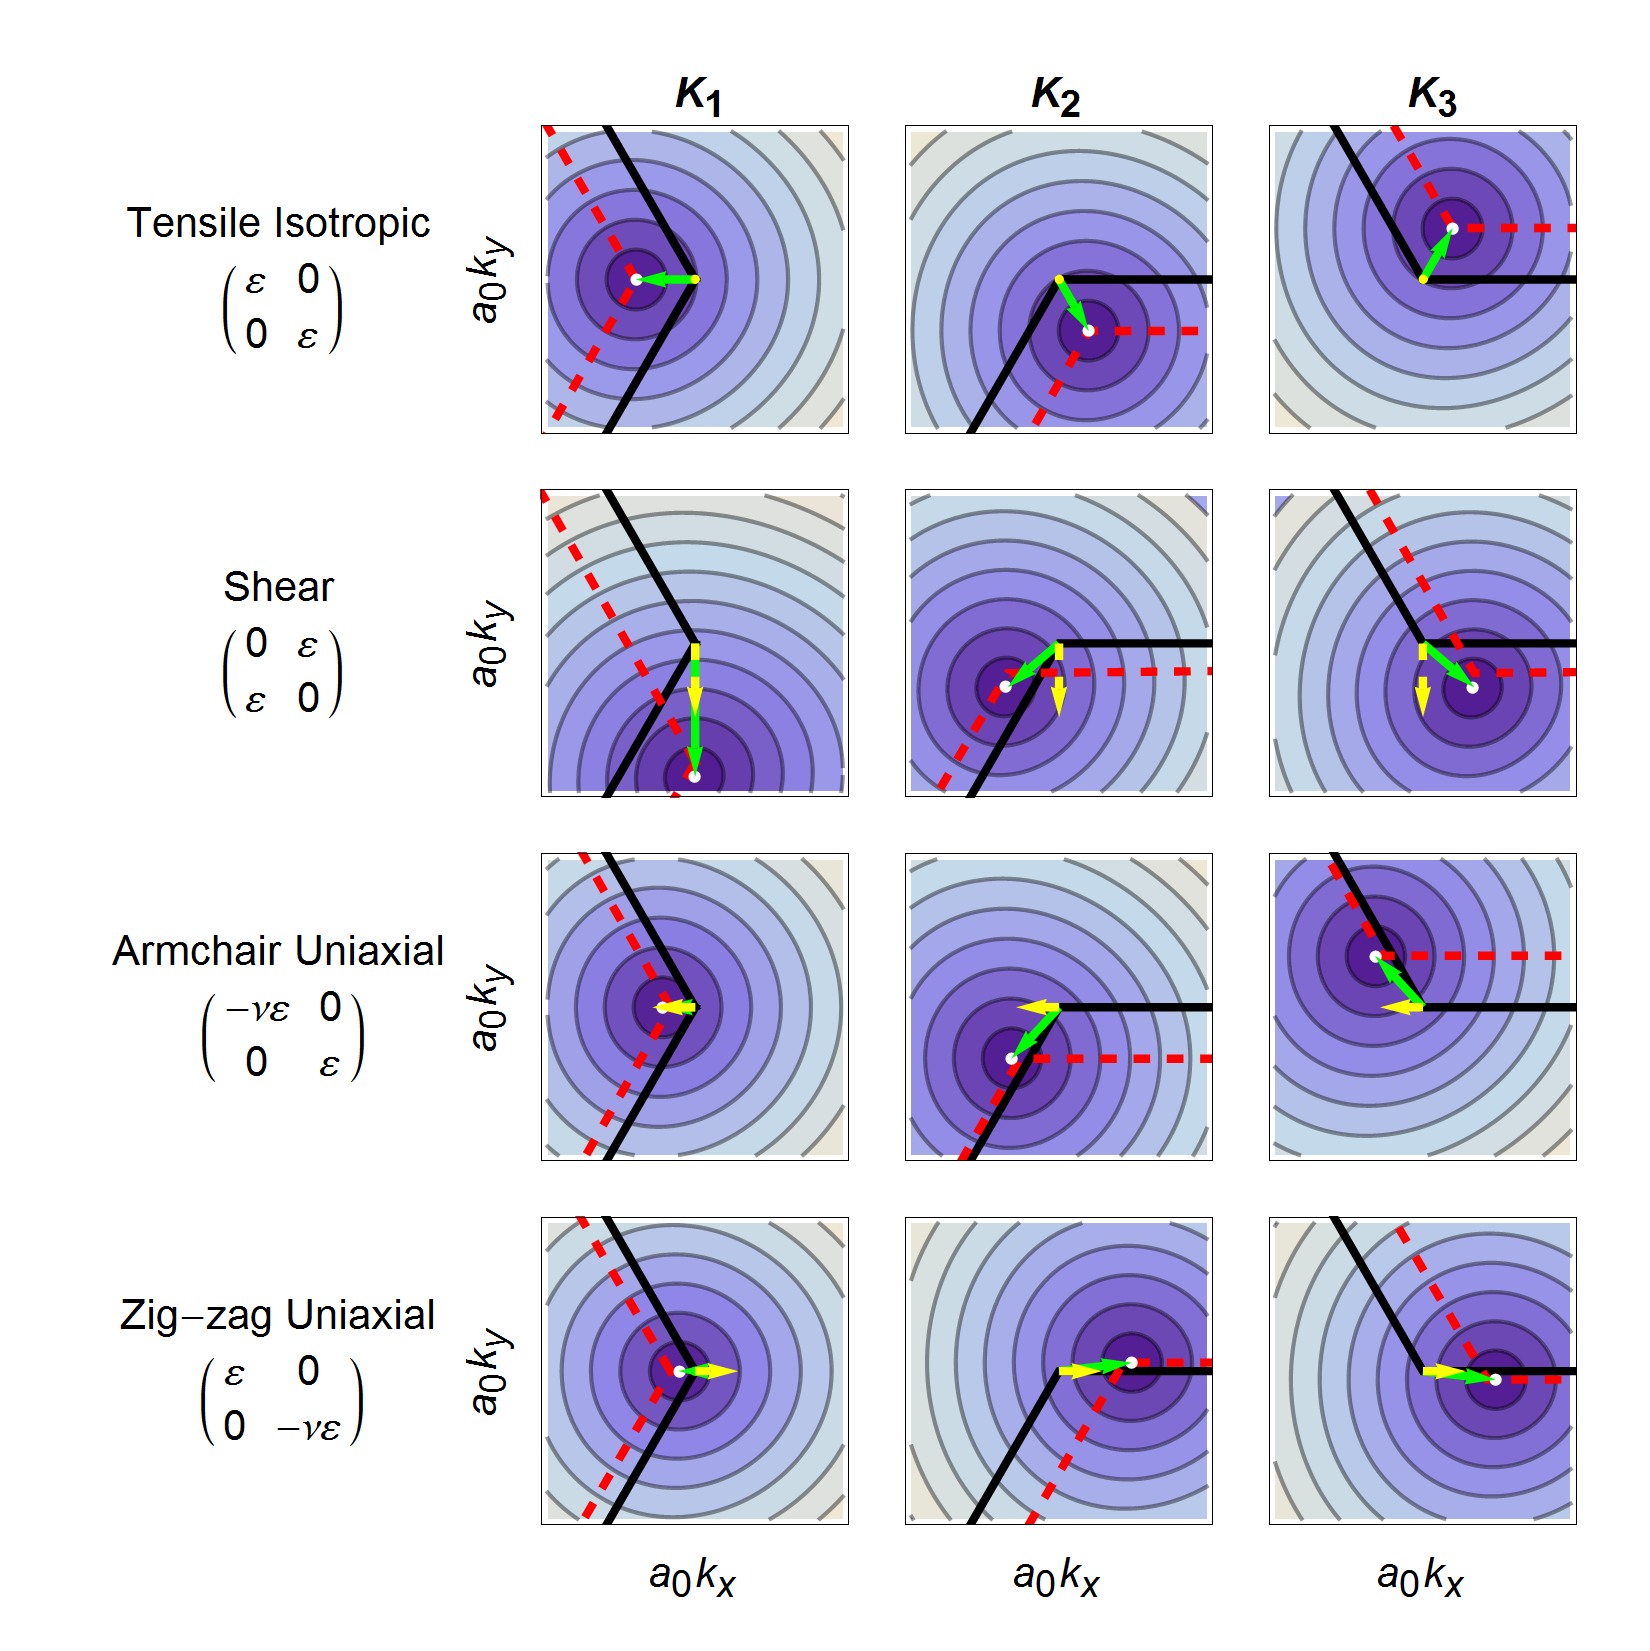
\includegraphics[scale=.75]{Figs_PVP/VPs.png}
  \end{center}
  \caption[A geometric depiction of the need for the corrections to the strain-induced pseudo vector potentials]{A geometric depiction of the need for the corrections to the strain-induced pseudo vector potentials.  Contours of the band structure of graphene under tensile isotropic strain, shear strain, armchair uniaxial strain, and zig-zag uniaxial strain (rows), for $\epsilon=1\%$ near the three $\bm{K}$ points (columns) are overlaid with the BZ of unstrained (solid, black)  and strained (dashed, red) graphene. Vectors mark the displacement of the Dirac points predicted by the traditional ($\vec{\mathcal{A}}_p$, dashed, yellow arrow) and the corrected ($\vec{\mathcal{A}}_{\bm{K}_{i}}$, solid, green arrow) form of the pseudo vector potential from Equations \ref{eq:PVP:PVP}, with the white dots marking the positions of the Dirac points for strained graphene. The yellow vectors appears as a dot for isotropic strain because the traditional form of the vector potential does not predict a shift in the Dirac points.  Each plot is square with an area of $0.12^2$. \label{fig:PVP:PVPshifts}}
\end{figure*}

In Figure \ref{fig:PVP:PVPshifts}, the reciprocal space shifts of the Dirac points predicted by the traditional and the corrected forms of the pseudovector potential are compared.
The contours represent the dispersion of strained graphene calculated using a nearest neighbor tight binding model which accounts for both the strain-induced changes in hopping amplitudes and the lattice deformation \cite{Pereira2009}.
The calculation of the shape of the strained BZ is described in Appendix \ref{chap:sBZ}.
For isotropic tensile strain, the lattice-corrected pseudo vector potential in Equation \ref{eq:PVP:PVP} properly predicts the displacement of each Dirac point due to strain.
The less trivial cases of uniaxial or shear strain are also shown in Figure \ref{fig:PVP:PVPshifts}.
The differences between the red (traditional) and orange (corrected) arrows make it clear that the lattice corrections are needed to determine the absolute position of the Dirac points in reciprocal space.

\section{Pseudo Magnetic Fields}
Having discussed the strain-induced analog of a real vector potential, the so called pseudo vector potential, it is natural to extend the analogy to pseudo magnetic fields.
Although Landau level quantization is usually associated with an out of plane magnetic field, it turns out that this field is not required in graphene.
In fact, Landau level quantization requires only the criterion used in deriving the pseudo vector potential: That there is a momentum shift which can be expressed as $\vec{p}-e\vec{A}$ where $\vec{p}$ is the momentum operator which obeys the canonical commutation relationship with the position operator $x$, $[x,p_x]=i \hbar$ \cite{Goerbig2011}.
It does not require a specific origin of $\vec{A}$.
Thus, strain alone can trick the electrons into quantizing into Landau levels as if they were in a magnetic field given by $\vec{B}=\vec{\nabla}\times\vec{\mathcal{A}}$.
This effect has recently been observed using scanning tunneling microscopy of accidentally strained graphene \cite{Levy2010,Yan2012,Yeh2011} and of engineered graphene analogs \cite{Gomes2012}.

This phenomenology is very powerful but has several subtleties.
First, it should be reiterated that despite the fact that the electrons act as if there were a real magnetic field, there is not one.
Strain does not somehow generate a magnetic field in a region near the graphene.
Second, strain can not break time reversal symmetry.
This symmetry is preserved via the relationship $\vec{\mathcal{A}}_{\bm{K_i}} = - \vec{\mathcal{A}}_{\bm{K_i'}}$ in Equation \ref{eq:PVP:PVP} which causes the pseudo magnetic field to point in opposite direction at time reversed $\bm{K}_i$ points.
An additional subtlety is the lacks of spatial dependence in the pseudo vector potential derived here.
If these calculations are treated as a local computation in the vicinity of position $\vec{r}$ then the spatial dependence of $\bm{\epsilon}$ and $\bm{\nabla u}$ provide the spatial dependence for $\vec{\mathcal{A}}(\vec{r})$ as long as this pseudomagnetic field is relatively constant on the scale of the magnetic length \cite{CastroNeto2009}.

The discussion of the pseudo magnetic field in the following sections begins with a discussion of the unimportance of the lattice corrections when calculating pseudo magnetic fields.
Next, a pressurized triangular graphene sealed microchamber \cite{Guinea2009} is used as an example to illustrate how pseudo magnetic fields might be engineered and measured.
This is followed by the prediction of a particularly interesting device, the hourglass shaped graphene sealed microchamber.
This device should have large localized pseudo magnetic fields which can be accessed using plasmonic field enhancement.
Finally, the importance of proper continuum modeling will be demonstrated by considering circular graphene sealed microchambers.

\subsection{Contribution of lattice corrections to the pseudo magnetic field}
Although the lattice corrections in Equation \ref{eq:PVP:PVP} are finite and, in general, have a position dependence, it happens that the lattice corrections to the pseudo vector potential do not effect the pseudo magnetic field.
This has been pointed out recently by de Juan \textit{et al.} \cite{DeJuan2013}. 
Using Equations \ref{eq:PVP:AfromH} and \ref{eq:PVP:nocurl} the pseudo vector potential from lattice corrections can be recast as 
\begin{equation*}
  \vec{\mathcal{A}}=-\frac{\hbar}{e} \bm{K}_i^{(')} \cdot \bm{\nabla u} 
  = - \frac{\hbar}{e} \vec{\nabla} \left( \bm{K_i^{(')}} \cdot \vec{u} \right) \ ,
\end{equation*}
where the order was changed using $K_j u_j \nabla_i=\nabla_i K_j u_j$.
Since the above is a total derivative, it cannot contribute to the pseudomagnetic field because $\nabla\times\nabla \phi \equiv 0$.
Thus, the only term in Equation \ref{eq:PVP:PVP} which contributes to the pseudo magnetic field is $\vec{\mathcal{A}}_p$.
As a result, even though the pseudo vector potential is different at the three $\bm{K}$ points, the pseudo magnetic field is the same at each $\bm{K}$ point and opposite in sign at the $\bm{K}'$ points.

The lattice corrections are still needed to correctly describe the shift in the positions of the Dirac points due to strain relative to a global frame of reference.
This includes the momentum-sensitive electronic tunneling to/from strained graphene from/to another system, probe, or contact \cite{Fogler2008}.

\subsection{Pressurized graphene sealed microchambers: Pseudo magnetic field test bed}
The potential of continuously replicating physics which usually only occurs at large magnetic fields is tantalizing.
Experimental measurements of pseudo magnetic fields \cite{Levy2010,Yan2012,Yeh2011,Gomes2012} have validated the theory and energized the idea of strain engineering.
However, to date no strain device has been predicted, fabricated, and then shown to have the desired properties.
The challenge now is to design and build devices which use this new science to enable unique device functionality.

This process of strain engineering pseudo magnetic field devices is non trivial from almost any stand point.
There are no established techniques for generating spatially varying strains in atomically thin materials.
In the past, graphene has deliberate been put under spatially uniform strain using strain transferred from an abutting polymer \cite{Yu2008,Ni2008,Tsoukleri2009,Huang2009,Mohiuddin2009,Frank2010,Yoon2011}, exfoliating graphene onto a piezoelectric substrate \cite{Ding2010,Jie2013}, or through the application of hydrostatic pressure \cite{Proctor2009,Clark2012}.
Generating specifically designed spatially varying strains, however, is a whole other ball game.
Since there are no predefined techniques for the device design, there are also no constraints provided to theorists to dictate what systems might be experimentally reasonable.
Identifying and specifying new methods of generating designed spatially varying strain is thus a major priority.
Beyond this challenge is the theoretical difficulty of the inverse problem.
The desired property, the pseudo magnetic field, is a function of the curl of the strain which is itself a function of the surrounding environment through continuum mechanics.
To complicate these non trivial mathematics is a general lack of understanding in how an atomically thin material, like graphene, responds to its surroundings.
All in all, there are several challenges which must be overcome before the Quantum Hall effect might be measured at room temperature with no magnetic field.

One early, experimentally accessible design which is predicted to yield fairly uniform pseudo magnetic fields is a pressurized triangular graphene sealed microchamber \cite{Guinea2009}.
To make the Landau levels as narrow and well defined as possible Guinea \textit{et al.} proposed a variety of designs for nearly uniform pseudo magnetic fields.
They noticed that strain profiles with an overall trigonal symmetry tend to generate smooth effective pseudomagnetic fields.
The pressurized graphene sealed microchamber represents the most experimentally realizable of their designs.
In this system equilateral triangle microchambers are etched into the underlying substrate and graphene is put across the top, sealing the gas inside.
When external pressure is applied the graphene is pushed into the microchamber generating a spatially varying strain which yields fairly uniform pseudo magnetic fields.

Shown in Figure \ref{fig:PVP:triangle} is the spatial distribution of the pseudo magnetic field for a graphene sealed equilateral triangle microchamber with 50 nm legs oriented along the zigzag direction pressurized to 14 MPa.
The pictured pseudo magnetic field is for the $\bm{K}$ points, the pseudo magnetic field for $\bm{K'}$ points would have the same magnitude but the opposite sign.
At this pressure the graphene sheet is under less than 0.26\% strain.
The pseudo magnetic fields are relatively large because the strains very quickly over the relatively small length scale of the device.

\begin{figure}
  \begin{center}
  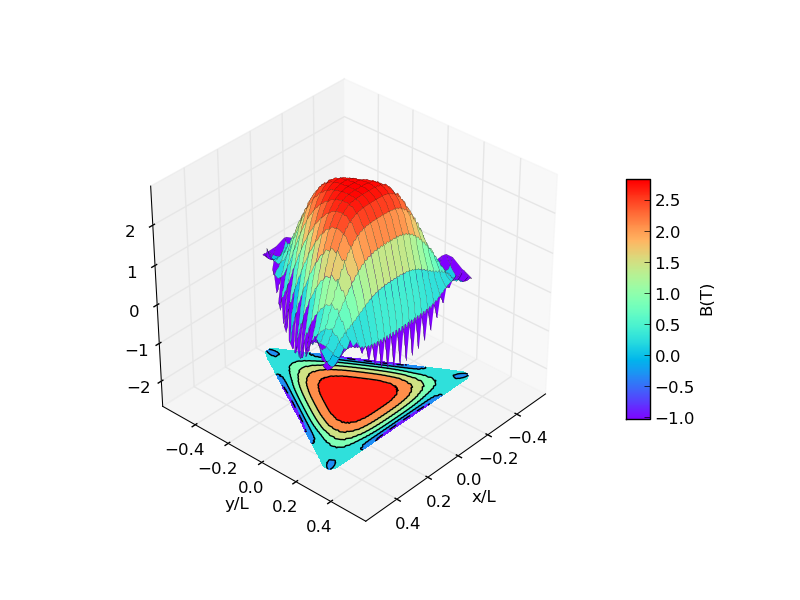
\includegraphics[scale=.75]{Figs_PVP/Triangle_PMF.png}
  \end{center}
  \caption[Pseudomagnetic field generated by pressurizing a triangular graphene sealed microchamber]{\label{fig:PVP:triangle} Pseudomagnetic field generated by pressurizing a triangular graphene sealed microchamber. A surface plot of the predicted spatial distribution of the pseudo magnetic field is shown above a contour plot with the same color scale. The equilateral triangular microchamber with edge lengths of 50 nm and a 2 nm fillets is pictured under 14 MPa of pressure. The graphene zigzag crystallographic orientation is in the $\hat{x}$ direction.}
\end{figure}

To generate this figure, the strain fields calculated using finite element analysis were used to calculate the spatial distribution of the pseudo vector potential from $\vec{\mathcal{A}}_p$ in Equation \ref{eq:PVP:PVP}.
Although $\vec{\mathcal{A}}_p$ was derived for the special case of in plane strains, it applies to out of plane strains as well.
This is because it is a function of the full Lagrangian strain tensor which properly references the deformation back to the undeformed coordinates.
Finally, the curl of $\vec{\mathcal{A}}_p$ is taken numerically to get the pseudo magnetic field.

Finite element analysis was performed using Comsol Multiphysics with a two-dimensional thin plate model including geometric non-linearity.
The edges were fixed and the pressure was applied using a face load.
Graphene's Young's Modulus of 1 TPa and thickness of 3.5 \AA \cite{Lee2008} were used along with the Poisson ratio of graphite of 0.165 \cite{Blakslee1970}.
To make the triangles more realistic 2 nm radius fillets were included on the corners to smooth the sharp boundaries.
The surface was meshed with triangles with a maximum element size of 1 nm and strain fields were evaluated in the mid-plane of the plate.

The importance of crystalographic orientation is illustrated by this triangular graphene sealed microchamber.
If the graphene is fixed while the microchamber is rotated underneath it, the pseudo magnetic field changes drastically.
Figure \ref{fig:PVP:Triangle_rot} compares the two extreme cases: The Zigzag edge along the legs of the triangle and the armchair edge along the legs of the triangle.
This 30 degree rotation ruins the large uniform pseudo magnetic field.
Thus, when fabricating these devices care need to be taken to orient the graphene in the appropriate direction.
One possible method to accomplish this is placing the graphene on an elastic polymer as an intermediate step.
This would allow the determination of the crystallographic orientation using the polarization dependence of the Raman strain response \cite{Huang2009}.
The graphene on polymer could be incorporated pick and place transfer technique which often use an intermediate polymer layer \cite{Dean2010,Zomer2011}.
Since different orientations can result in such different physics one should consider all crystal orientations when theoretically modeling a device.

\begin{figure}
  \begin{center}
  \begin{tikzpicture}
	\node at (2.75 cm,0)  {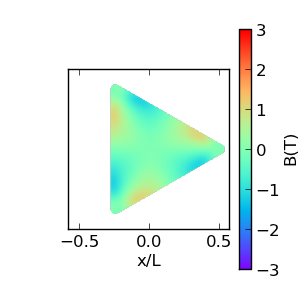
\includegraphics{Figs_PVP/Rotate_30.png}};
	\node at (-2.75 cm,0) {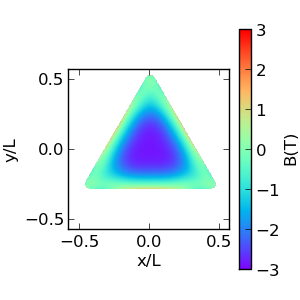
\includegraphics[trim=0 0 1.75cm 0,clip=true]{Figs_PVP/Rotate_0.png}};

	\path (-2.5 cm, 3) node{\textbf{a:} Zigzag oriented} ++ (5 cm,0) node{\textbf{b:} Armchair oriented};
\end{tikzpicture}
  \end{center}
  \caption[The effects of crystallographic orientation on the pseudo magnetic field]{\label{fig:PVP:Triangle_rot} The effects of crystallographic orientation on the pseudo magnetic field for equilateral triangle graphene sealed microchambers with 50 nm legs and 2 nm fillets under 14 MPa of applied pressure. The zig zag crystallographic orientation is along the $\hat{x}$ direction for both plots and both plots are referenced to the same color bar.  In (a) and (b) the underlying microchamber is rotated such that the legs of the triangle are along the zigzag and armchair directions respectively.}
\end{figure}

Graphene sealed microchambers define a class of strain engineered devices which could provide a test bed for strain engineering.
Even though graphene sealed microchambers do not possess the well defined electrical current path needed for electronic devices, they should still be useful as a strain engineering test bed.
They represent an experimentally realizable method of generating measurable pseudo magnetic fields.
Since similar devices have been made in the past, it is believable that they can be fabricated.
In fact, micron sized graphene sealed microchambers are used in the study of how graphene slides presented in Chapter \ref{chap:fri}.
Additionally the Landau levels should be measurable using optical probes or local probes such as scanning tunneling spectroscopy.
In particular, due to electron phonon coupling the phonon energy measured by Raman spectroscopy is renormalized when this energy matches specific Landau level transitions \cite{Goerbig2011}.
These magneto phonon resonances have been observed on multilayer epitaxial graphene \cite{Faugeras2009}, on single layer graphene like regions on the surface of graphite crystals \cite{Faugeras2011}, and for CVD graphene on SiO$_2$ \cite{Kim2013}.
Thus, it is easy to envision an experiment where a graphene sealed microchamber is pressurized while the Raman spectrum is measured \emph{in situ}.
Monitoring these energy fluctuations as the pseudo magnetic field is tuned by changing the applied pressure would provide an experimental test of the predicted pseudo magnetic fields.

In summary, pressurized graphene sealed microchambers represent a unique test bed for studying pseudo magnetic field effects.
The strain distributions can be easily treated theoretically using finite element analysis, the predicted devices are experimentally realizable, and the resulting pseudo magnetic fields could be measured with optical techniques such as Raman spectroscopy.

\subsection{Large, localized pseudo magnetic fields in plasmonically enhanced regions}
Microchambers with different shapes were simulated using the same technique as for equilateral triangles.
The predicted pseudo magnetic field distributions for simple convex shapes including circles, squares, rectangles, hexagons, and acute triangles were not compelling.
Concave devices, however, proved much more interesting.
When the graphene bends around a tip, the strain fields change rapidly causing large but localized pseudo magnetic fields.
Usually such a localized effect would be difficult to measure optically.
However, the tip has a second function.
It can enhance an optical field making the local effects measurable.
If the optical field enhancement region and the region of large pseudo magnetic field were to overlap, Raman spectroscopy could be used to directly probe the high field regions. 

An hourglass shaped device yields a near perfect agreement between the location of the plasmonic field enhancement and the regions of large pseudo magnetic fields.
The hourglass device and plasmonic response is illustrated in Figure \ref{fig:PVP:hourglass_Plas}.
The field enhancement, modeled by Arif \c{C}etin, was modeled using a 3-dimensional finite difference time domain technique.
Devices would consist of a periodic, two dimensional array of the unit cell shown in (a) and (b).
In this way, any graphene sheet would cover multiple devices, increasing the signal.
The unwanted signal from the supported graphene between hourglasses is minimized by destructive interference of the incident and emitted light upon reflection off the gold substrate.
Device geometry, detailed in (a) and (b), was chosen so that the plasmon resonance wavelength, shown in (c), was in an experimentally accessible region.
The dielectric function of the metallic layers are obtained from Palik \cite{Palik1985}.
The predicted reflectivity in (c) was found using a power reflection monitor located 1 $\mu m$ from the structure.
In (d) the field enhancement of the device for light polarized in the x direction is shown.
It is calculated using a field monitor located at the top surface of the top gold layer.
The Raman enhancement goes as the square of the intensity enhancement since the intensity of the incident light and the intensity of the inelastically scattered light are both enhanced.
The resulting Raman enhancement is greater than $5 \times 10^5$ in the region extending roughly 2 nm away from the tips.
As a result, the signal measured from these tiny regions should be 3 orders of magnitude stronger than the signal from the rest of the hourglass.

\begin{figure}
  \begin{center}
  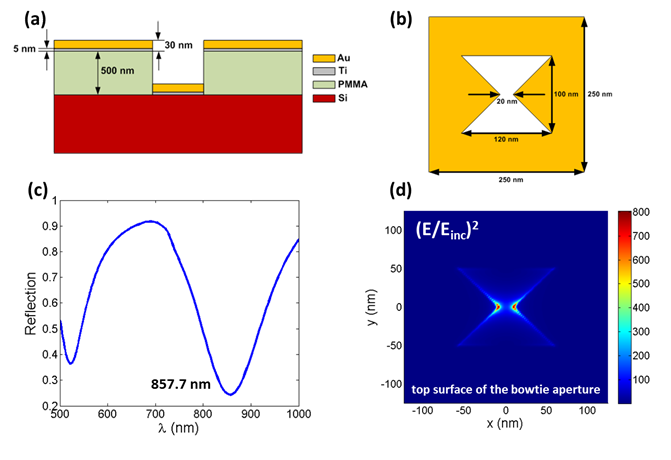
\includegraphics[scale=.75]{Figs_PVP/HourGlass_Plasmonics.png}
  \end{center}
  \caption[The design and plasmonic response of the hourglass device]{\label{fig:PVP:hourglass_Plas} The design and plasmonic response of the hourglass device.  The drawings in (a), the side view, and (b), the top view, detail the geometry of one unit cell of the plasmonic device. In (c) the predicted spectral reflectivity of the device is plotted.  The intensity enhancement at the top surface of the device is plotted in (d).}
\end{figure}

The pseudo magnetic field distribution resulting from sealing the microchambers shown in Figure \ref{fig:PVP:hourglass_Plas} with graphene and applying 14 MPa of pressure is shown in Figure \ref{fig:PVP:hourglass_PMF}.
The pseudo magnetic fields reach the impressive value of 60 Tesla near the tip.
This small region of large pseudo magnetic field is made experimentally accessible by the plasmonic field enhancement.
When compared, the region of high pseudo magnetic field and the regions of large field enhancement are almost indistinguishable.
This should allow for the measurement of pressure tunable, very large pseudo magnetic fields using Raman spectroscopy.

\begin{figure} 
  \begin{center}
  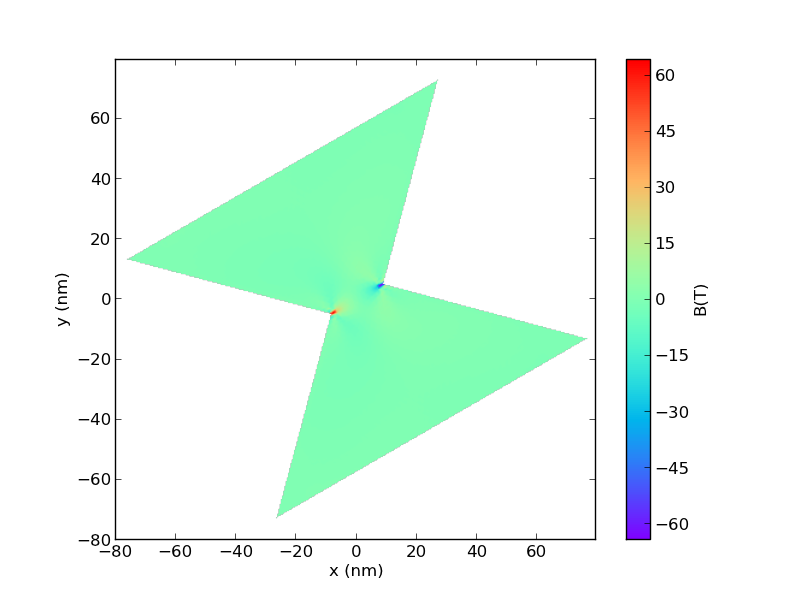
\includegraphics[scale=.75]{Figs_PVP/HourGlass_PMF.png}
  \end{center}
  \caption[Large pseudo magnetic fields near the corners of a pressurized hourglass graphene sealed microchamber]{\label{fig:PVP:hourglass_PMF} Large pseudo magnetic fields near the corners of a pressurized hourglass graphene sealed microchamber are visible in the image plot of the predicted pseudo magnetic fields. The microchamber is formed by the union of two right triangles. This leaves two 90 degree tips separated by 20 nm. The device is pressurized to 14 MPa of pressure. The graphene zigzag crystallographic orientation is in the $\hat{x}$ direction.}
\end{figure}

\subsection{The necessity of proper continuum modeling\label{sec:PVP:GoodCont}}
The first step toward modeling pseudo magnetic fields is the difficult task of determining the expected strains.
This is complicated for several reasons.
First, the large deflection of thin plates is often a difficult nonlinear problem.
Second, many well accepted approximate continuum models are not valid for pseudo magnetic fields.
Historically, most works sought approximations that accurately determined aspects of the deflection profile, sacrificing the accuracy of the strain profile in the process.
Models that do not correctly predict the strain distribution can not be used to predict pseudo magnetic fields.
Finally, the form of the interactions between atomically thin sheets and their surrounding environment is not yet completely understood.
As a result, calculating strains can be a tricky task.

Pressurized circular graphene sealed microchambers illustrate the pitfalls of improper continuum modeling.
The symmetry of the system makes analytic solutions for the strain possible.
In fact, there are several different models of increasing accuracy which can be compared.
The pseudo magnetic field for each is calculated from the curl of the vector potential which contributes to the pseudo magnetic field, $\vec{\mathcal{A}}_p$ in Equation \ref{eq:PVP:PVP}, 
\begin{equation*}
\vec{\mathcal{A}}_{p,cyl}=\frac{\phi_0}{2a} \frac{\beta}{2 \pi}
  \left( \begin{array}{c}
    (\epsilon_{\rho\rho}-\epsilon_{\phi,\phi}) cos(3\phi)-2 \epsilon_{\rho,\phi} sin (3 \phi) \\
    -(\epsilon_{\rho\rho}-\epsilon_{\phi,\phi}) sin(3\phi)-2 \epsilon_{\rho,\phi} cos (3 \phi)
  \end{array} \right) \ ,
\end{equation*}
where $\vec{\mathcal{A}}_{p,cyl}$ is in cylindrical coordinates.

The spatial distributions of pseudo magnetic fields predicted using three different continuum models are shown in Figure \ref{fig:PVP:circle}.
For each continuum model a surface plot of the pseudo magnetic field is plotted above a contour plot.
The boundary of each plot is positioned at the point where the strains, and thus the pseudo magnetic fields, go to zero.
In Figures \ref{fig:PVP:circle}a and \ref{fig:PVP:circle}b the plots terminates at the edge of the circular microchamber whereas in \ref{fig:PVP:circle}c the plot extends further because in this case the strain is allowed to spread to the supported graphene.
From left to right the strain distributions used as input become more accurate.
In each model the microchamber has a radius of 100 nm and is put under 70 MPa of pressure.

\begin{figure}
  \begin{center}
  \newcommand{\circscale}{.85}
\begin{tikzpicture}[scale=\circscale]
	% Unscaled scale=.2
	\node at (-3 cm, 0){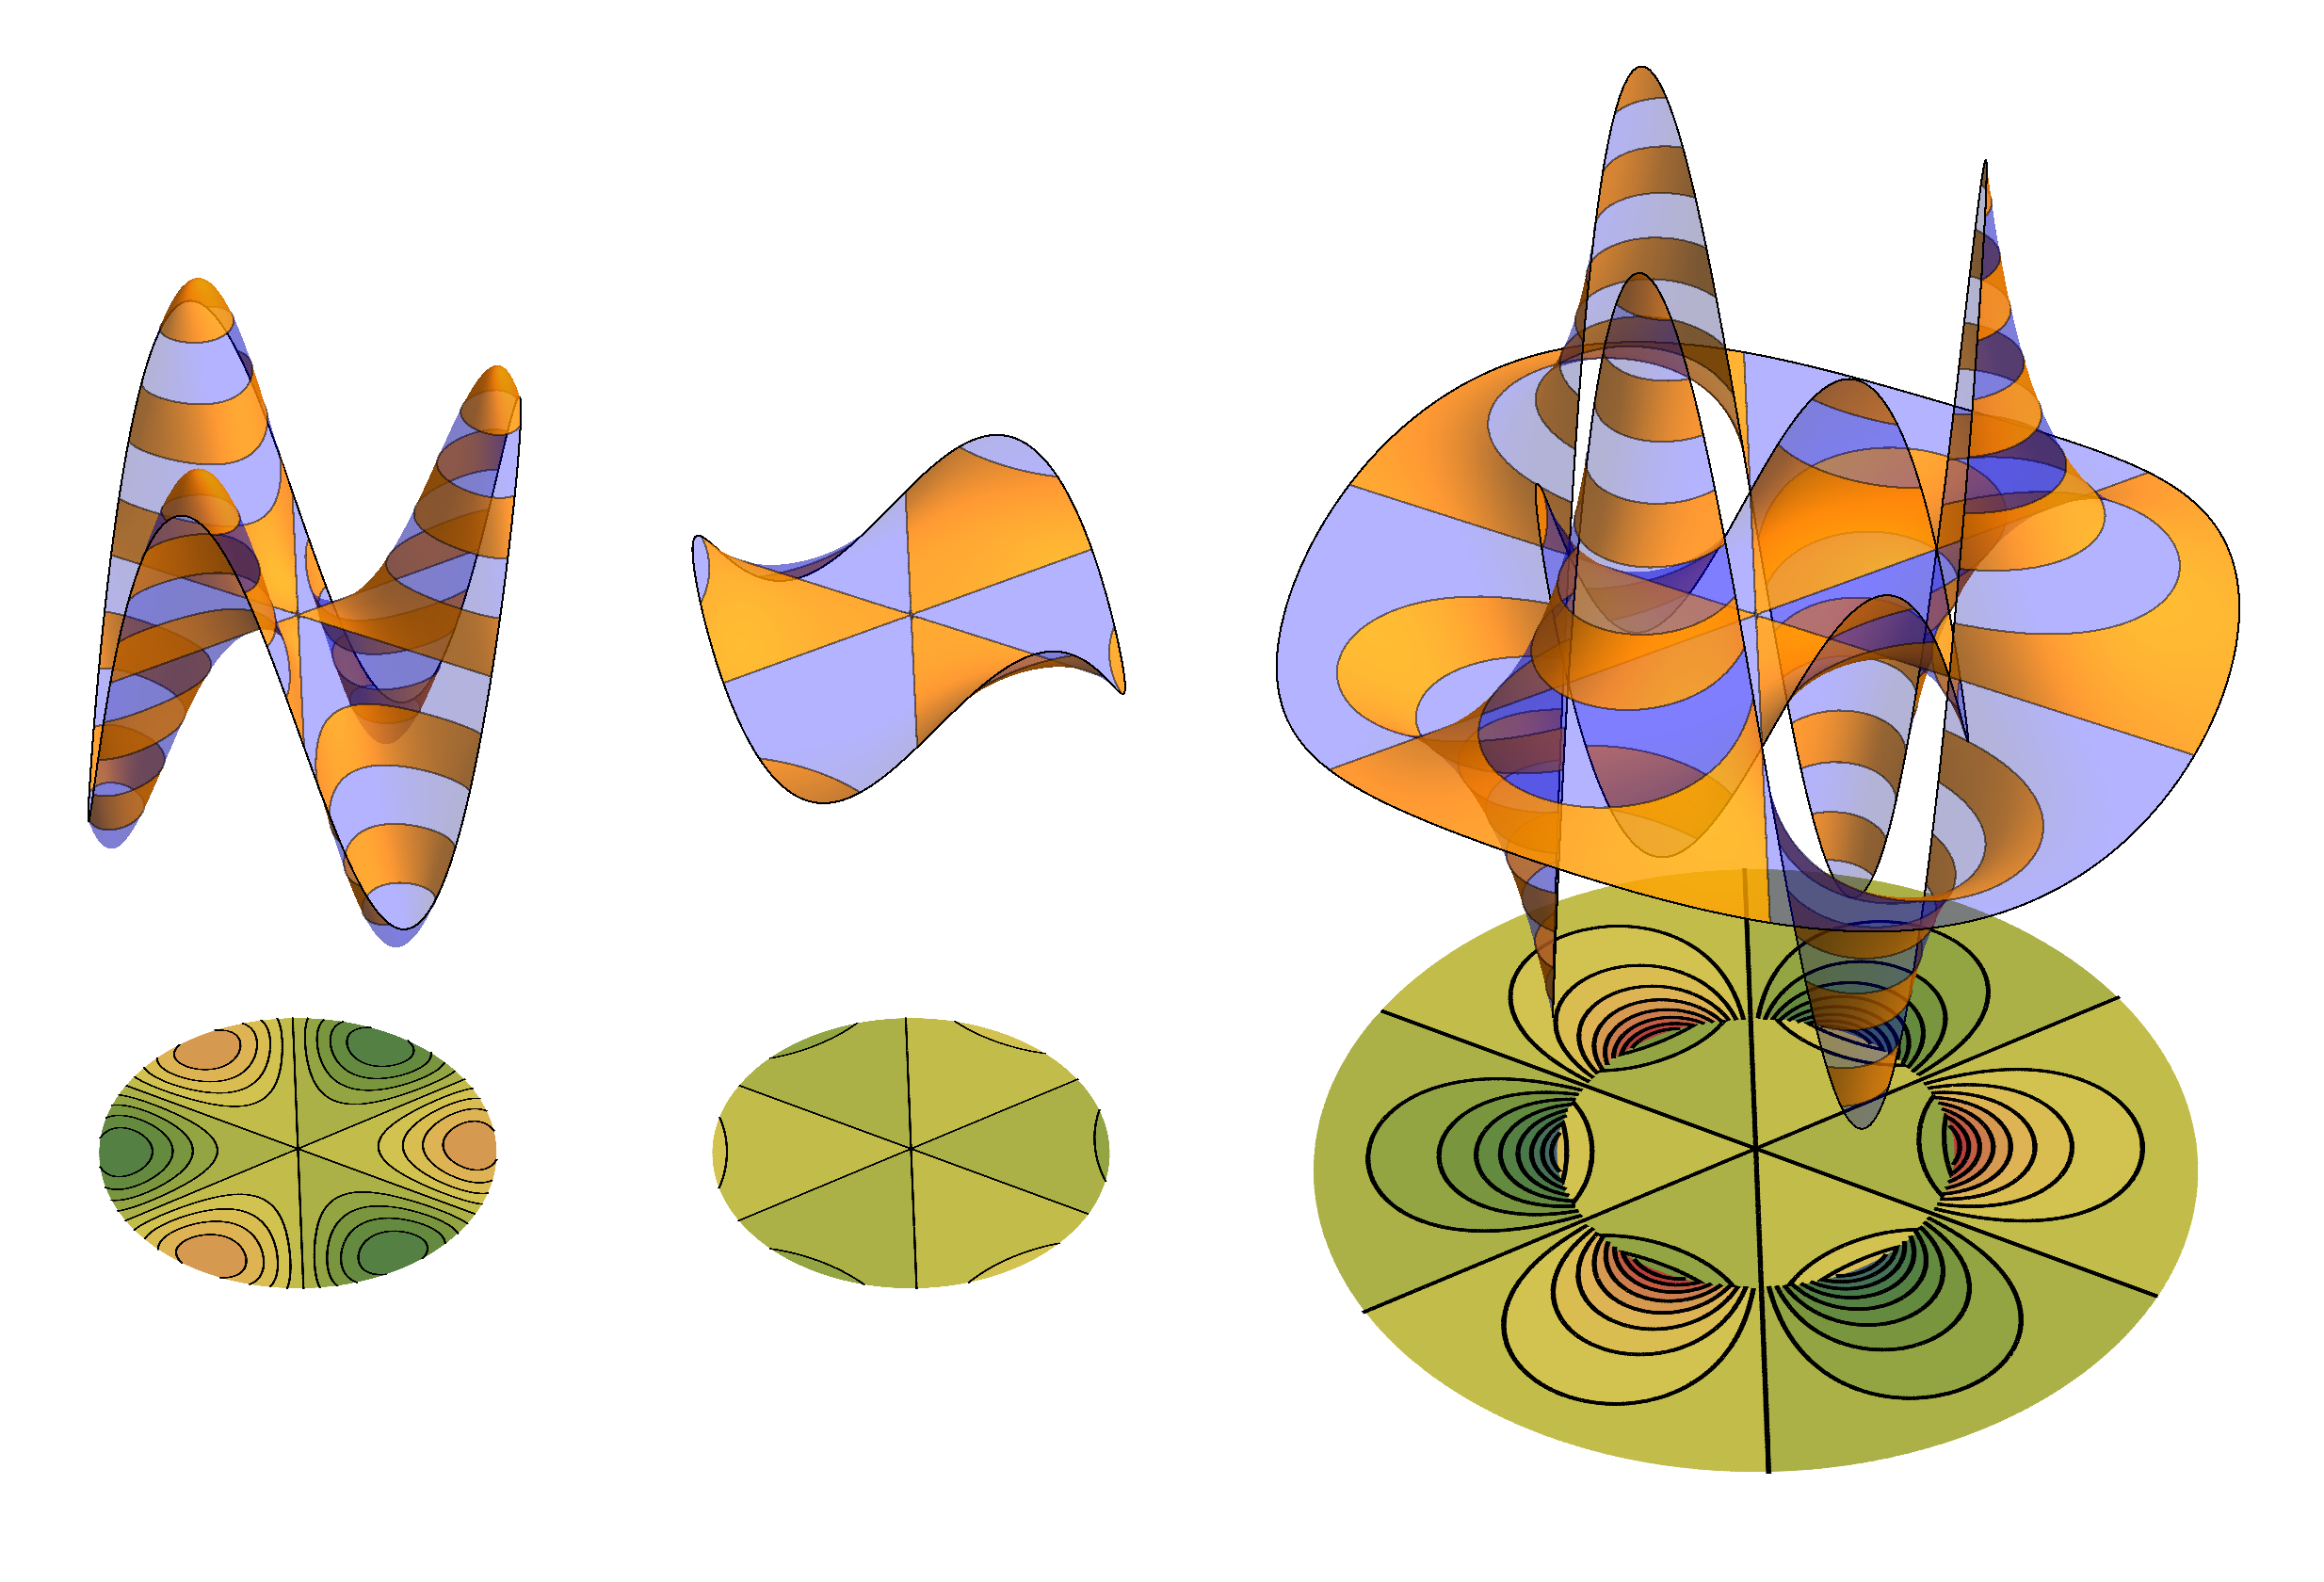
\includegraphics[scale=.17]{Figs_PVP/Circle_PMF.png}};
	\node at (5 cm,-1 cm){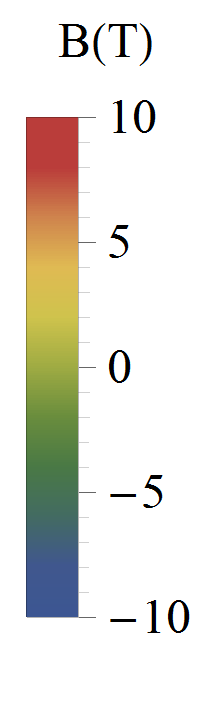
\includegraphics[scale=\circscale]{Figs_PVP/Circle_PMF_Bar.png}};

	\path (-9,4) node{\textbf{(a)}} ++ (3.5cm,0) node{\textbf{(b)}} ++ (3.5cm,0) node{\textbf{(c)}};
\end{tikzpicture}
  \end{center}
  \caption[Different pseudo magnetic field distributions resulting from three different models]{\label{fig:PVP:circle} Different Pseudo magnetic field distributions resulting from three different models of a 100 nm radius circular graphene sealed microchamber pressurized to 70 MPA. The spatial distribution of the pseudo magnetic field for each model is illustrated using a surface plot with 1 Tesla bands plotted above a contour plot referenced to the color bar on the right. The z scale and the in plane scale are the same for each plot.  For each model the pseudo magnetic field at the center is zero. In (a) the strains are determined using a small strain continuation model \cite{Timoshenko}, in (b) Hencky's model \cite{Hencky1915} is used, and in (c) the extended Hencky model derived in Chapter \ref{chap:fri} is used with a sliding friction of 31.5 MPa.  The radial extent of (c) is larger because the extended Hencky model allows the strain to be distributed to the supported graphene.}
\end{figure}

The strain distribution used in Figure \ref{fig:PVP:circle}a is based on an approximate solution useful for interpreting bulge tests.
In this popular approximation the large deflection lateral displacement is assumed to have the same form as that of the small deflection limit \cite{Timoshenko}.
This simple model provides everything needed to determine the Young's modulus of a thin film based on the pressure induced deflection at the center: A relationship between pressure, Young's modulus, and the center deflection.
However, this approximation does not accurately describe the strain profiles and so is not applicable for studying pseudo magnetic fields.
Nonetheless, Kyung-Joong Kim \textit{et al.} use a similar model to predict exotic physical phenomena in pressurized circular graphene sealed microchambers \cite{Kim2011b}.
As shown in Figure \ref{fig:PVP:circle}a, when this model is naively used three distinct global maximum and three distinct global minimum are visible with pseudo magnetic fields of nearly 5 Tesla.
The six fold symmetry is a reflection of the lattice symmetry.

In Figure \ref{fig:PVP:circle}b Hencky's model is used to predict the pseudo magnetic field.
This model is an exact series solution for the large deflection of a circular plate under a uniform vertical load with fixed boundaries.
Although more complicated, this model should accurately describe the strains in the system as long as the boundaries are held fixed.
The resulting pseudo magnetic fields are noticeably reduced, barely exceeding 1 Tesla.
In this case the peaks occur at the boundary of the microchamber.

Finally, in \ref{fig:PVP:circle}c the pseudo magnetic fields are calculated using the extended Hencky model that is derived and experimentally confirmed in Chapter \ref{chap:fri}.
In this model the fixed boundary conditions at the edge of the microchamber are relaxed.
The supported graphene is allowed to slide against a resistive frictional force.
The frictional force for this small of a device at this large of a pressure have not yet been measured experimentally.
To get a qualitative idea of the changes resulting from sliding, the dimensionless frictional force found in Chapter \ref{chap:fri} by comparison to atomistic modeling of a 6 nm radius microchamber was used.
The resulting strain distribution of the suspended graphene is similar to the one predicted by the Hencky model.
The strain distribution in the supported graphene, however, is much different.
Since the derivative of the strain is not continuous at the edge of the microchamber, nether is the pseudo magnetic field.
In fact, since the slope of the radial strain changes sign, so does the psuedo magnetic field.
As friction decreases the distributed strain the pseudo magnetic field of the supported graphene decays to zero from its value of almost 9 Tesla at the edge of microchamber.

The example of cylindrical graphene sealed microchambers clearly shows that the validity of predicted pseudo magnetic fields is directly tied to the validity of the strain distribution predicted by the continuum model.
One needs to be careful to ensure that the approximations made in solving for the large deflection of the plate do not make the resulting strain distributions inaccurate.
Further, one has to be careful to accurately account for how the graphene interacts with its environment.

\section{Conclusion}
The pseudo vector potential was derived in full and new, $\bm{K}_i$ point dependent corrections to the pseudo vector potential were found.
Even though these correction do not contribute to the pseudo magnetic field, they are necessary to complete the analogy between strain-induced momentum shifts and a real vector potential.
Additionally, these shifts are required to accurately determine the position of the Dirac points and should be taken into account when considering electrical transport over a strain boundary.

Sealed microchambers were discussed as a test bed for predicting and measuring pseudo magnetic fields.
It was shown that an hour glass microchamber should generate very large pseudo magnetic fields while also enabling their measurement through plasmonic enhancement.
Finally, the need for accurate continuum modeling was demonstrated using cylindrical microchambers as an example.